% TBP on Cu(111)
\label{sec:single-TBP-Cu111}
\begin{wrapfigure}{r}{5cm}\centering
	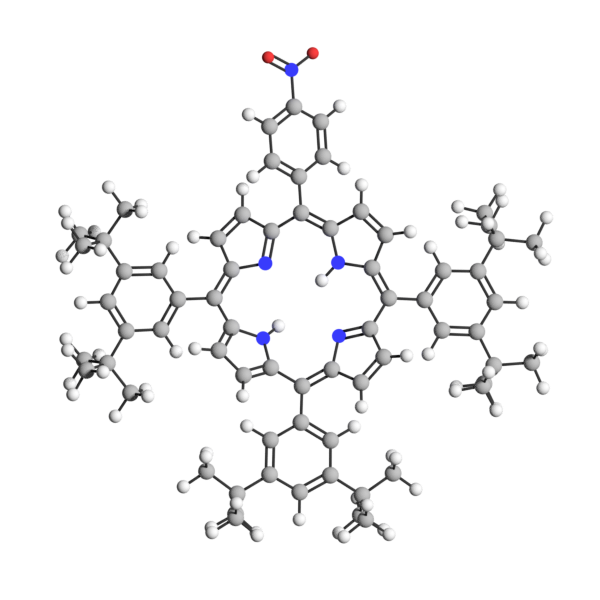
\includegraphics[angle=90, width=5cm]{./images/molecules/max-zoom/TBP-single-600}
	\caption{TBP with three di-tert-butyl and a single nitro phenyl group added at the meso position.}
	\label{fig:}
\end{wrapfigure}
When adsorbed at room temperature, TBP distributes equally on the surface, forms unordered islands and decorates step edges. Molecules orient their main axis (connecting line from one di-tert-buytl-phenyl ring across the center to the nitrophenyl ring) along the dense packed substrate rows most often, less are \SI{15}{\degree} of \textcolor{red}{\textbf{((Refer to image?))}}. Several binding motifs (as shown in \autoref{fig:binding-motifs-TBP-Cu111}) are observed, namely
\begin{itemize}
 \item A dimer, where molecules lie ``head-to-head'', functional groups ($NO_2$) pointing at each other
 \item A ``triangle'', where molecules are rotated \SI{120}{\degree} and functional groups point towards a shared center. Although this motif does not occur very often (or at least under very flexible angles), it is given as an example where the functional groups point to each other. Similar motifs (like 3 molecules in \SI{90}{\degree} are observed together with other orientations. 
 \item Chains with different length appear, where the nitro group of molecule 1 points to the di-tert-butyl group of molecule 2 (``head-to-tail''). At the connection points, molecules appear brighter, promoting a physical overlap of the two molecules.
\end{itemize}

Center-center distances are typically \SI{1.78}{\nano \meter} (for the head-to-tail) and \SI{1.5}{\nano \meter} for the head-to-head connection. 

\begin{figure}[]
	\centering
	\subfigure[Overview image]{
		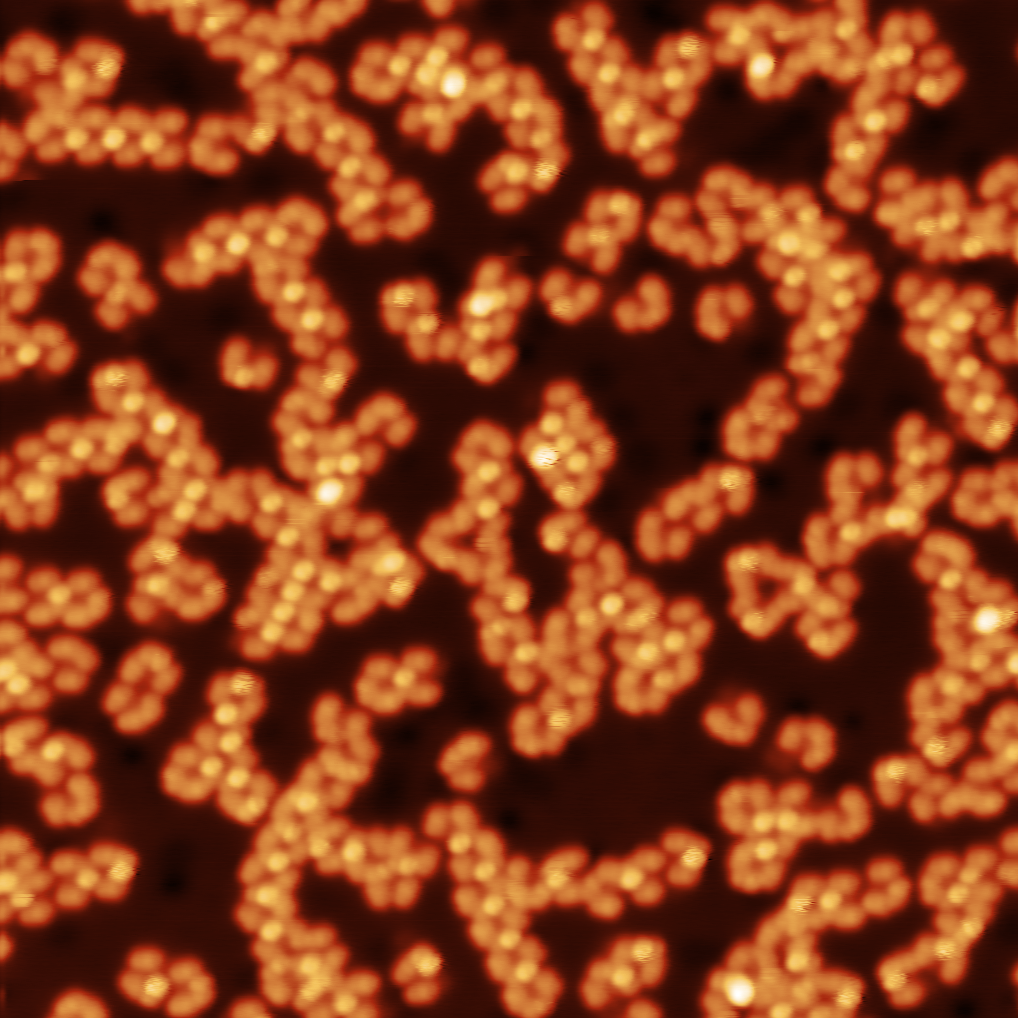
\includegraphics[width=0.7\textwidth]{./images/F151128-083339-44nm}
		\label{fig:single-TBP-cu111-overview}
	}
	
	\subfigure[Monomer]{
		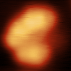
\includegraphics[width=0.22\textwidth]{./images/F151128-083339-monomer-3nm.png}
		\label{fig:single-TBP-cu111-monomer}	
	}
	\subfigure[Chain]{
		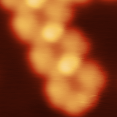
\includegraphics[width=0.22\textwidth]{./images/F151128-083339-chain-5nm}
		\label{fig:single-TBP-cu111-chain}	
	}
	\subfigure[Dimer]{
		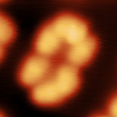
\includegraphics[width=0.22\textwidth]{./images/F151128-083339-dimer-5nm.png}
		\label{fig:single-TBP-cu111-dimer}	
	}
	% \subfigure[Model representation of the binding motifs. See text for more details.]{
	%  \includegraphics[width=0.4\textwidth]{./images/TBP-motivs-on-Cu111}
	% }
	\caption{RT adsorbed single nitro functionalized TBP on Cu(111) and their most abundant binding motifs. \subref{fig:single-TBP-cu111-overview} Each of the binding motif can be found as well in the overview STM data, as well as in the enlarged images (b-d). All images recorded with \SI{-500}{\milli\volt}, \SI{0.1}{\nano\ampere}, color scale \SIrange{0}{300}{\pico\meter}. Image width: \subref{fig:single-TBP-cu111-overview} \SI{44}{\nano\meter}, 
		\subref{fig:single-TBP-cu111-monomer} \SI{3}{\nano\meter}, 	
		\subref{fig:single-TBP-cu111-chain} \& 
		\subref{fig:single-TBP-cu111-dimer} \SI{5}{\nano\meter}
	}
	\label{fig:binding-motifs-TBP-Cu111}
\end{figure}

\paragraph{``head-to-head''}
To model the occurring binding motifs, deformations of the molecules have to be taken into account. Because nitro groups face each other in the ``head-to-head'' connection, their distance would be to small to facilitate a similar binding mechanism like for the TPCN on copper (where copper surface ad atoms promote binding between nitrogens), so no free space between the facing nitro groups is observed. Because the distance is so small, the phenyl ring (with attached nitro group) rotates by \SI{45}{\degree}, to make the phenyl ring stand upright. When the second molecule does the same, both match each other with negligible lateral shift, reproducing the STM images best. Similar binding motivs are reported in \cite{kato_dispersive_2008} for non-covalent cross linking of dicarboxylic acids in hydrogels. Although the situation on a metal-surface may change considerably (only 2D - no 3D, metal present - will change chemistry), the observed binding motif matches very well.

\paragraph{``head-to-tail''}
The chain motif ``head-to-tail'' is reconstructed using the unique contrast of the TBP molecule. When the center-center distance is measured, molecules are modeled that distance away from each other. These models show a physical overlap between molecules, which in not possible because of steric hindrance. To solve the problem, the nitro-group (head) of one molecule if rotated by \SI{35}{\degree} out of the plane (like pulling the nitro-group upwards, not rotating the group left/right). 

%---------------- models bauen und bsp bilder einf\"ugen.  ---------------- 

\paragraph{Flexible tert-butyl-groups}
\begin{figure}\centering
	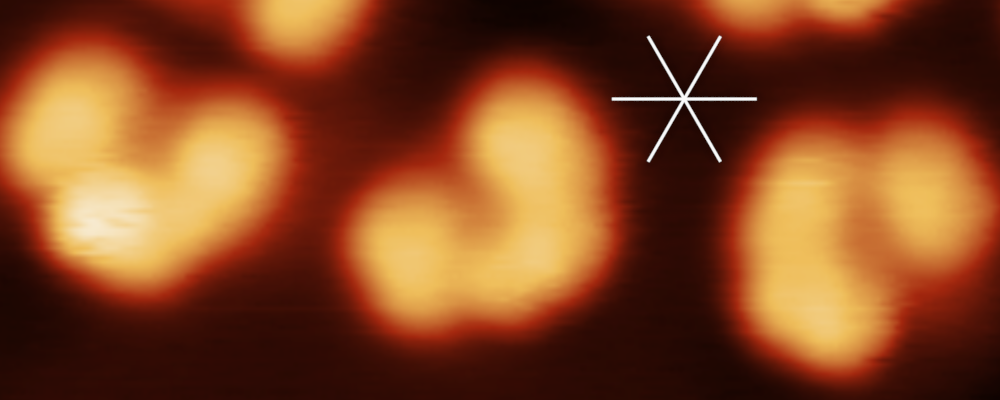
\includegraphics[width=0.44\textwidth]{./images/F151128-083339-10x4-overlay.png}
	\caption{Different appearances of TBP on Cu(111). While most of monomers (center in image above) show even heights with their tert-butyl functions, some (left) do posses an elevated tert-butyl group. The orientation of the tert-butyl groups is aligned with the high symmetry crystal direction (indicated by white lines) most often. Image recorded with  \SI{-500}{\milli\volt}, \SI{0.1}{\nano\ampere}. Image width: \SI{10}{\nano \meter}}
	\label{fig:TPB-butyl-flexibility-SMT}
\end{figure}

Another interesting fact is that butyl groups of TBP seem to orient them self (as far as steric hindrance allows for) along the dense packed rows of the copper substrate. Again, one has to be careful when reconstructing geometrical information from STM images. Like the distortion of legs in the TPCN molecule, this rotation can be explained by a rotation of single butyl groups. Although the phenyl ring remains at the same position/rotation, tert-butyl groups are allowed to rotate such that they appear in different heights. Because STM (constant current) follows equipotential lines, the whole phenyl-di-tert-butyl-complex looks rotated in plane, although it may not be. This is confirmed in literature\cite{heim_surface-assisted_2010, heim_self-assembly_2010}.

%%%%%%%%%%%%%%%%%%%%%%%%%%%%%%%%%%%%%%%%%%%%%%%%%%%%%%%%%%%%%%%%%%%%%%%%%%%%%%%%%%